\newpage
\section{Logic}

\subsection{Block definition diagram}
Blokdiagrammer giver et indblik på den overordnede strukturen af \textit{Konditioneringsapparatet}.  Hver kasse skal ses som en del der indgår i systemet \\
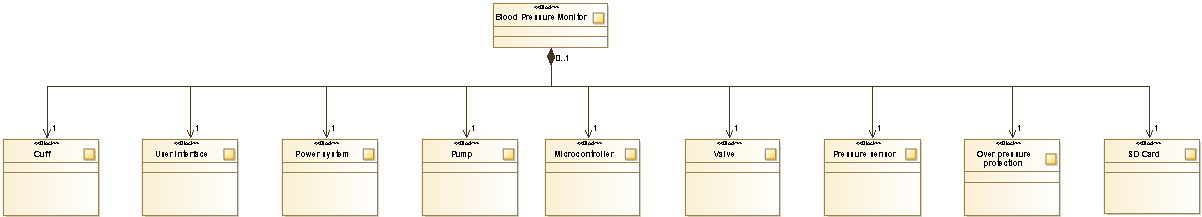
\includegraphics[width=\textwidth]{pdfs/BD-crop.pdf}

\subsection{Domænemodel}
Diagrammer beskriver det systemet som helhed. Ved gennemgang af alle use cases findes væsentlig navneord og disse oprettet som konceptuelle klasser. Det konceptuelle klasser er derefter oversat til engelsk \\
\begin{figure}[H]
	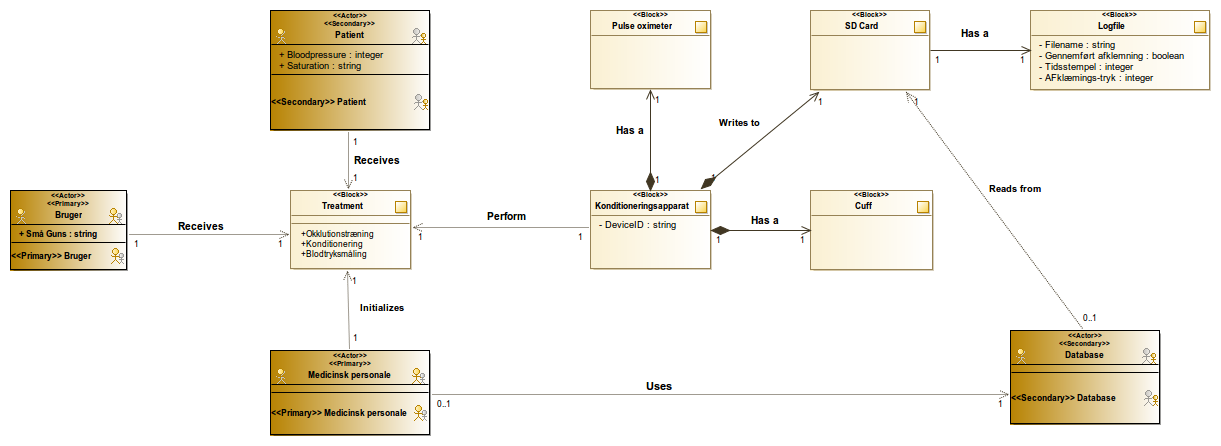
\includegraphics[width=\textwidth]{pdfs/DomainModel.png}
	\caption{Block definition diagram over \textit{Konditioneringsapparatet}}
\end{figure}


\newpage
\subsection{State machine diagram}
\subsubsection{Boot}
\begin{figure}[H]
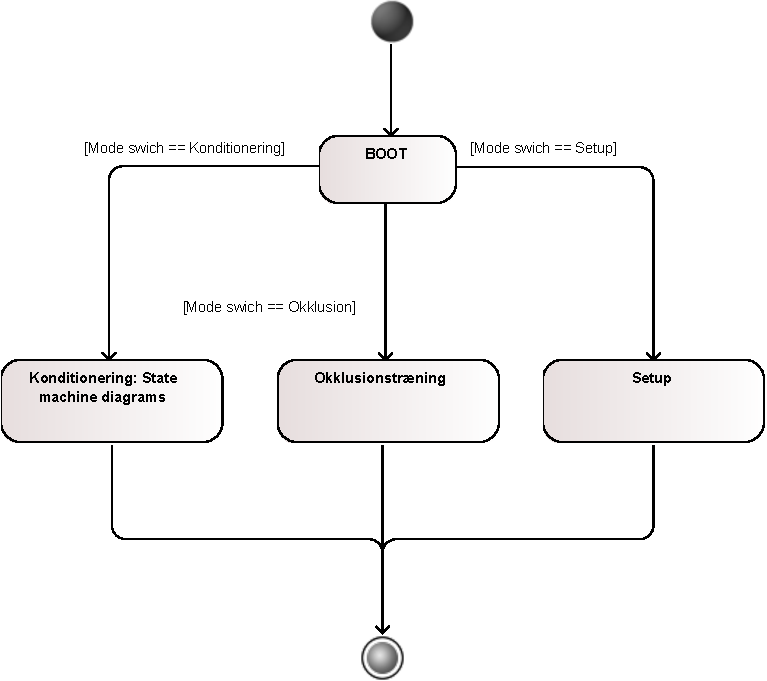
\includegraphics[width=\textwidth]{pdfs/STM_BOOT-crop.pdf} 
\caption{}
\end{figure}

\newpage
\subsubsection{Konditionering}
Ved knap tryk på [Start/Stop] \\
\begin{figure}[H]
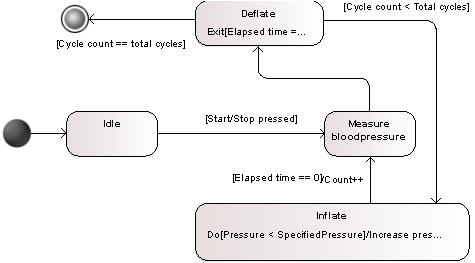
\includegraphics[width=\textwidth]{pdfs/STM_Konditionering1-crop.pdf}
\caption{State machine diagram over Konditioneringsforløb}
\end{figure}

Ved knap tryk på [Mål blodtryk] \\
\begin{figure}[H]
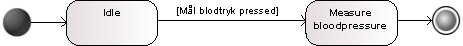
\includegraphics[width=\textwidth]{pdfs/STM_Konditionering2-crop.pdf}
\caption{State machine diagram over blodtryksmåling}
\end{figure}
\newpage

\subsubsection{Okklusion}

	\begin{figure}[H]
		\begin{center}
		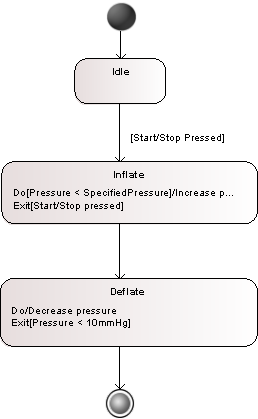
\includegraphics[width=0.5\textwidth]{pdfs/STM_Okklusion-crop.pdf}
		\caption{State machine diagram over okklusionsforløb}
	\end{center}
	\end{figure}

\newpage

\subsubsection{Setup}
\begin{figure}[H]
	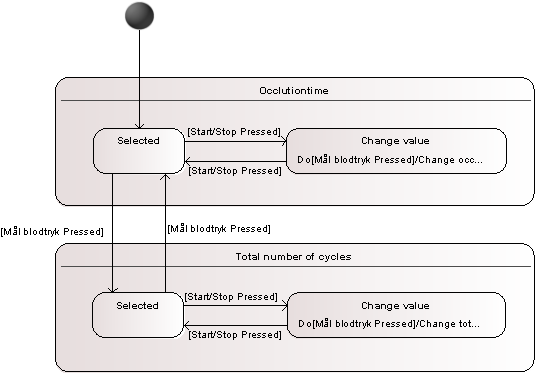
\includegraphics[width=\textwidth]{pdfs/STM_Setup-crop.pdf}
	\caption{State machine diagram over setup forløbet}
\end{figure}

